\documentclass[aspectratio=43]{beamer}
% Theme works only with a 4:3 aspect ratio
\usetheme{CSCS}

\usepackage{tikz}
\usepackage{pgfplots}
\usepackage{pgfplotstable}
\usetikzlibrary{pgfplots.groupplots,spy,patterns}
\usepackage{listings}
\usepackage{color}
\usepackage{tcolorbox}
\usepackage{anyfontsize}
\usepackage{xspace}
\usepackage{graphicx}

% define footer text
\newcommand{\footlinetext}{CUDA Introduction}

% Select the image for the title page
\newcommand{\picturetitle}{cscs_images/image5.pdf}

% fonts for maths
\usefonttheme{professionalfonts}
\usefonttheme{serif}

% source code listing
\newcommand{\axpy}{{\ttfamily axpy}\xspace}
\newcommand{\extra}{{\bfseries extra}:\xspace}
%\newcommand{\lst}[1]{\colorbox{white!90!blue}{\lstinline!#1!}}
\newcommand{\lst}[1]{\colorbox{white!20!black}{\lstinline!#1!}}
\newcommand{\lstfont}[1]{\color{#1}\scriptsize\ttfamily}
\newcommand{\lsttinyfont}[1]{\color{#1}\fontsize{7}{7}\ttfamily}
\newcommand{\lstinlinefont}[1]{\color{#1}\scriptsize\ttfamily}
\newcommand{\todo}[1]{\color{red}{TODO:}\color{blue}{ #1}}

% set indent to a more reasonable level (so that itemize can be used in columns)
\setlength{\leftmargini}{20pt}

%\lstset{
%    language=[ANSI]C++,
%    basicstyle=\lstinlinefont{blue!30!black},
%    breaklines=true
%}

\lstset{
    language=[ANSI]C++,
    showstringspaces=false,
    backgroundcolor=\color{white!10!black},
    basicstyle=\lstfont{white},
    identifierstyle=\lstfont{white},
    keywordstyle=\lstfont{magenta!40!white},
    numberstyle=\lstfont{white},
    stringstyle=\lstfont{cyan},
    commentstyle=\lstfont{yellow!30!white},
    moredelim=[is][\lstfont{green!50!white}]{@}{@},
    emph={
        cudaMalloc, cudaFree,
        cudaMallocHost, cudaFreeHost,
        cudaMemcpyAsync, cudaMemcpy, cudaMemcpyHostToDevice, cudaMemcpyDeviceToHost,
        cudaSuccess, cudaGetLastError, cudaGetErrorString,
        cudaErrorMemoryAllocation, cudaError_t,
        cudaOccupancyMaxPotentialBlockSize,
        __global__, __shared__, __device__, __host__,
        __syncthreads,
        cudaEvent_t, cudaStream_t,
        cudaEventCreate, cudaEventSynchronize, cudaEventDestroy,
        cudaEventElapsedTime, cudaEventQuery, cudaEventRecord,
        cudaStreamWaitEvent,
        threadIdx, blockIdx, blockDim, gridDim,
        cudaStream_t, cudaStreamCreate, cudaStreamDestroy,
        cudaMemcpyDeviceToDevice, cudaMemcpyHostToHost,
    },
    emphstyle={\lstfont{green!50!white}},
    breaklines=true
}

\definecolor{codenumber}{rgb}{0.5,0.5,0.5}
\definecolor{codekeyword}{rgb}{0.9,0.4,0.7}
\definecolor{codeCUDA}{rgb}{1.0,0.6,0.6}

\lstdefinestyle{boxcuda}{
    language=[ANSI]C++,
    showstringspaces=false,
    backgroundcolor=\color{white!10!black},
    basicstyle=\lstfont{white},
    identifierstyle=\lstfont{white},
    keywordstyle=\lstfont{magenta!40!white},
    numberstyle=\lstfont{white},
    stringstyle=\lstfont{cyan},
    commentstyle=\lstfont{yellow!30!white},
    moredelim=[is][\lstfont{green!50!white}]{@}{@},
    emph={
        cudaMalloc, cudaFree,
        cudaMallocHost, cudaFreeHost,
        cudaMemcpyAsync, cudaMemcpy, cudaMemcpyHostToDevice, cudaMemcpyDeviceToHost,
        cudaSuccess, cudaGetLastError, cudaGetErrorString,
        cudaErrorMemoryAllocation, cudaError_t,
        cudaOccupancyMaxPotentialBlockSize,
        __global__, __shared__, __device__, __host__,
        __syncthreads,
        cudaEvent_t, cudaStream_t,
        cudaEventCreate, cudaEventSynchronize, cudaEventDestroy,
        cudaEventElapsedTime, cudaEventQuery, cudaEventRecord,
        cudaStreamWaitEvent,
        threadIdx, blockIdx, blockDim, gridDim,
        cudaStream_t, cudaStreamCreate, cudaStreamDestroy,
        cudaMemcpyDeviceToDevice, cudaMemcpyHostToHost,
    },
    emphstyle={\lstfont{green!50!white}},
    breaklines=true
}

\lstdefinestyle{boxcudatiny}{
    language=[ANSI]C++,
    showstringspaces=false,
    backgroundcolor=\color{white!10!black},
    basicstyle=\lsttinyfont{white},
    identifierstyle=\lsttinyfont{white},
    keywordstyle=\lsttinyfont{magenta!40!white},
    numberstyle=\lsttinyfont{white},
    stringstyle=\lsttinyfont{cyan},
    commentstyle=\lsttinyfont{yellow!30!white},
    moredelim=[is][\lsttinyfont{green!50!white}]{@}{@},
    emph={
        cudaMalloc, cudaFree,
        cudaMallocHost, cudaFreeHost,
        cudaMemcpyAsync, cudaMemcpy, cudaMemcpyHostToDevice, cudaMemcpyDeviceToHost,
        cudaSuccess, cudaGetLastError, cudaGetErrorString,
        cudaErrorMemoryAllocation, cudaError_t,
        cudaOccupancyMaxPotentialBlockSize,
        __global__, __shared__, __device__, __host__,
        __syncthreads,
        cudaEvent_t, cudaStream_t,
        cudaEventCreate, cudaEventSynchronize, cudaEventDestroy,
        cudaEventElapsedTime, cudaEventQuery, cudaEventRecord,
        cudaStreamWaitEvent,
        threadIdx, blockIdx, blockDim, gridDim,
        cudaStream_t, cudaStreamCreate, cudaStreamDestroy,
        cudaMemcpyDeviceToDevice, cudaMemcpyHostToHost,
    },
    emphstyle={\lstfont{green!50!white}},
    breaklines=true
}

\DeclareTextFontCommand{\emph}{\bfseries\color{blue!70!black}}

% Please use the predifined colors:
% cscsred, cscsgrey, cscsgreen, cscsblue, cscsbrown, cscspurple, cscsyellow, cscsblack, cscswhite

\author{Ben Cumming, CSCS}
\title{CUDA: Introduction and API}
\subtitle{}
\date{\today}

\begin{document}

% TITLE SLIDE
\cscstitle

% TABLE OF CONTENT SLIDE
% All options for table of contents:
% currentsection, currentsubsection, firstsection=xx, hideallsubsections, hideothersubsections, part=xx, pausesections, pausesubsections, sections=xx, sections={xx-yy}, sections={xx,yy}
%\cscstableofcontents[hideallsubsections]{Title}

% CHAPTER SLIDE
\cscschapter{Introduction}

%%%%%%%%%%%%%%%%%%%%%%%%%%%%%%%%%%%%
\begin{frame}[fragile]{}
%%%%%%%%%%%%%%%%%%%%%%%%%%%%%%%%%%%%
    \begin{info}{The plan}
        \begin{itemize}
            \item learn about the GPU memory model
            \item implement parallel CUDA kernels for simple linear algebra
            \item learn how to scale our parallel kernels to utilize all resources on the GPU
            \item understand which types of workloads can best take advantage of GPU resources
            \item learn about thread cooperation and synchronization in CUDA
            \item learn about concurrent task-based parallelism with CUDA
            \item learn how to use MPI in CUDA applications
        \end{itemize}
    \end{info}

\end{frame}

%%%%%%%%%%%%%%%%%%%%%%%%%%%%%%%%%%%%
\begin{frame}[fragile]{}
%%%%%%%%%%%%%%%%%%%%%%%%%%%%%%%%%%%%
    \begin{info}{Prerequisites for the course}
        \begin{itemize}
            \item no GPU or graphics experience required
            \item I assume C++ knowledge
            \begin{itemize}
                \item I will be using C++11 (the bits that make C++ easier!)
                \item there is no native CUDA implementation for Fortran
                \begin{itemize}
                    \item there is a CUDA Fortran provided by PGI, however it is not widely used.
                \end{itemize}
                \item Fortran users are encouraged to work with a C++ user for the practical exercises
            \end{itemize}
            \item the generic GPU programming concepts in the CUDA part will be useful for people interested in OpenACC
        \end{itemize}
    \end{info}

\end{frame}

%%%%%%%%%%%%%%%%%%%%%%%%%%%%%%%%%%%%
\begin{frame}[fragile]{}
%%%%%%%%%%%%%%%%%%%%%%%%%%%%%%%%%%%%
    \begin{info}{CUDA language is a superset of C++}
        \begin{itemize}
            \item write CPU code using C++ (C++11 since CUDA 6.5)
            \item keywords for writing tasks to be executed by GPU threads (kernels)
            \item use special syntax for launching tasks/kernels on GPU
        \end{itemize}
    \end{info}

    \begin{info}{CUDA is GPU-specific}
        \begin{itemize}
            \item the CUDA language extensions define the \emph{programming model}
            \item features map directly to hardware (e.g. shared memory, thread blocks)
        \end{itemize}
    \end{info}

    \begin{info}{CUDA toolkit is more than just a language}
        \begin{itemize}
            \item runtime library for managing GPU resources
            \item tools for profiling and debugging
        \end{itemize}
    \end{info}
\end{frame}


%%%%%%%%%%%%%%%%%%%%%%%%%%%%%%%%%%%%
\begin{frame}[fragile]{}
%%%%%%%%%%%%%%%%%%%%%%%%%%%%%%%%%%%%
    \begin{info}{What about the GPU in my laptop/desktop/cluster?}
        \begin{itemize}
            \item the GPUs in Piz Daint are NVIDIA Tesla K20X devices
            \item Tesla devices are high-end products with features required for high-performance computing
            \begin{itemize}
                \item high double precision performance (1.2 TFlops)
                \item large DRAM (6 GB)
                \item ECC memory
            \end{itemize}
            \item the K20X Tesla cards use the Kepler architecture
            \begin{itemize}
                \item some features are not supported by older cards
            \end{itemize}
            \item I focus on features of the K20X devices for this course
        \end{itemize}
    \end{info}

\end{frame}

%%%%%%%%%%%%%%%%%%%%%%%%%%%%%%%%%%%%
\begin{frame}[fragile]{}
%%%%%%%%%%%%%%%%%%%%%%%%%%%%%%%%%%%%
    \begin{columns}[T]
        \begin{column}{0.4\textwidth}
            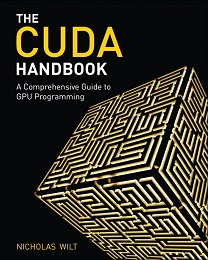
\includegraphics[width=\textwidth]{./images/CUDA-Handbook-Cover208_260.jpg}
        \end{column}

        \begin{column}{0.6\textwidth}
            \begin{info}{recommended reading}
                \textbf{\small CUDA Handbook: A Comprehensive Guide to GPU Programming}
                \begin{itemize}
                    \item  Nicholas Wilt
                    \item  released in 2013
                    \item  detailed coverage of everything you need to know
                    \item  lots of example codes and micro-benchmarks
                \end{itemize}
            \end{info}
        \end{column}
    \end{columns}
    \begin{center}
    \end{center}
\end{frame}

%%%%%%%%%%%%%%%%%%%%%%%%%%%%%%%%%%%%
\cscschapter{Working with GPU memory}
%%%%%%%%%%%%%%%%%%%%%%%%%%%%%%%%%%%%


%%%%
\begin{frame}[fragile]{}
    \begin{center}
        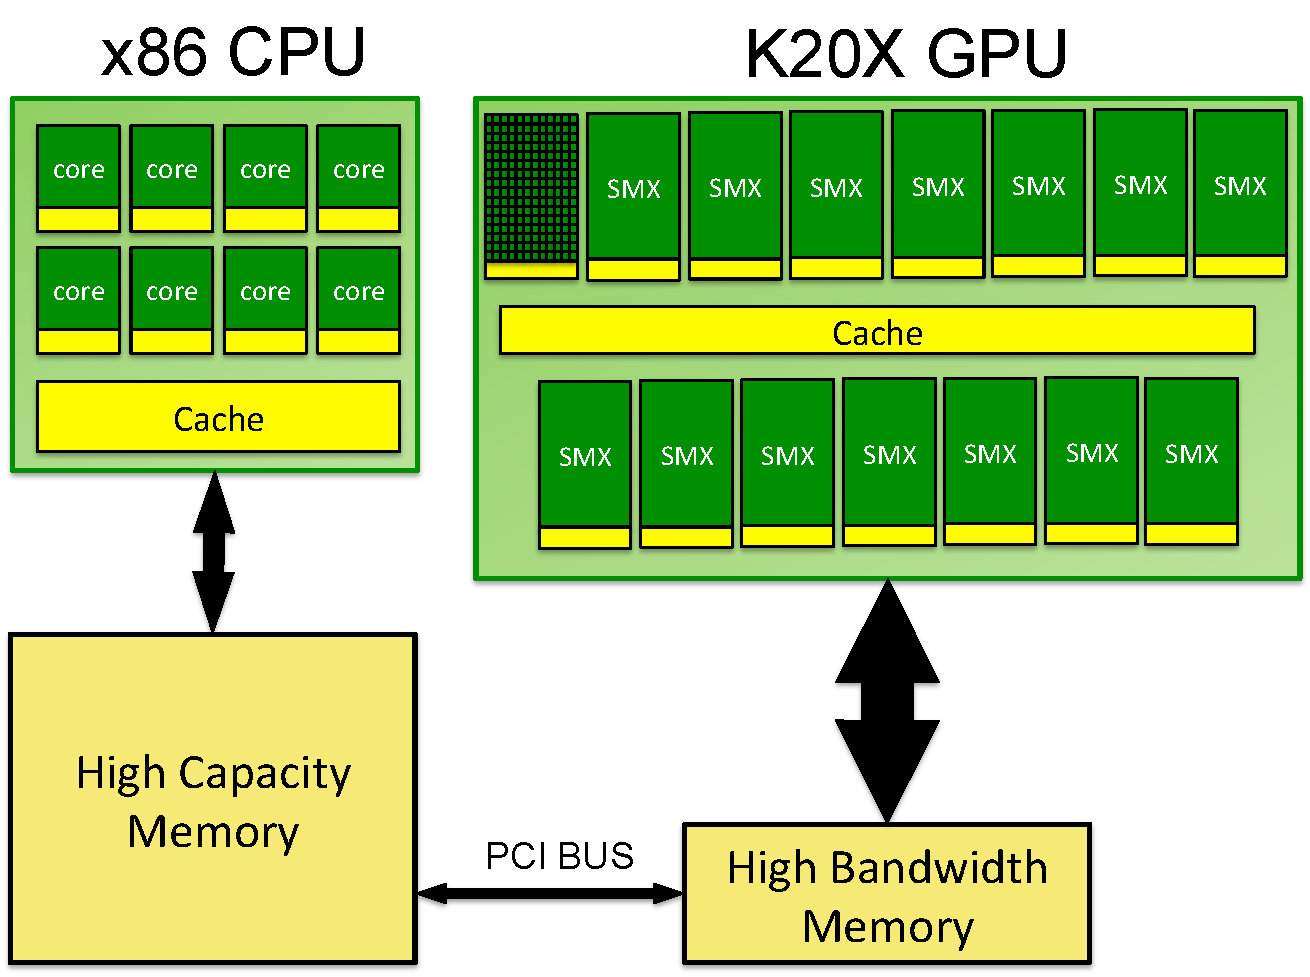
\includegraphics[width=0.9\textwidth]{./images/node.pdf}
    \end{center}
\end{frame}

%%%%%%%%%%%%%%%%%%%%%%%%%%%%%%%%%%%%
\begin{frame}[fragile]{}
%%%%%%%%%%%%%%%%%%%%%%%%%%%%%%%%%%%%
    \begin{info}{Host and device have separate memory spaces}
        \begin{itemize}
            \item data must be copied between host and device memory via PCI
            \item data must be in device memory for kernels to access
                \begin{itemize}
                    \item not strictly true\ldots
                    \item but a strict requirement for high performance
                \end{itemize}
            \item ensure data is in the right memory space \emph{before} computation starts
            \begin{itemize}
                \item PCIe2 = 6-12 GB/s
                \item CPU socket = 35-50 GB/s
                \item K20X  = 180 GB/s
            \end{itemize}
        \end{itemize}
    \end{info}

\end{frame}

%%%%%%%%%%%%%%%%%%%%%%%%%%%%%%%%%%%%
\begin{frame}[fragile]{}
%%%%%%%%%%%%%%%%%%%%%%%%%%%%%%%%%%%%
    \begin{info}{CUDA uses C pointers to reference GPU memory}
        \centering \lst{double *data = // pass an address to either host or device memory}
        \begin{itemize}
            \item a pointer can hold an address in \emph{either} device or host memory
            \item accessing a device pointer in host code, or vice versa, is \emph{undefined behaviour}
            \item we have to take care that we know which memory space a pointer is addressing
        \end{itemize}
        The CUDA runtime library provides functions that can be used to allocate, free and copy device memory
    \end{info}

\end{frame}

%%%%%%%%%%%%%%%%%%%%%%%%%%%%%%%%%%%%
\begin{frame}[fragile]{}
%%%%%%%%%%%%%%%%%%%%%%%%%%%%%%%%%%%%
    \begin{info}{Allocating device memory}
        \centering \lst{cudaMalloc(void **ptr, size_t size)}
    \begin{itemize}
        \item \lst{size} number of bytes to allocate
        \item \lst{ptr} points to allocated memory on exit
    \end{itemize}
    \end{info}

    \begin{info}{Freeing device memory}
        \centering \lst{cudaFree(void *ptr)}
    \end{info}

    \begin{code}{Allocate memory for 100 doubles on device}
%..................................
        \begin{lstlisting}[style=boxcuda]
double *v; // C pointer that will point to device memory
auto size_in_bytes = 100*sizeof(double);
cudaMalloc(&v, size_in_bytes); // allocate memory
cudaFree(v);                   // free memory
\end{lstlisting}
%..................................
    \end{code}
\end{frame}

%%%%%%%%%%%%%%%%%%%%%%%%%%%%%%%%%%%%
\begin{frame}[fragile]{}
%%%%%%%%%%%%%%%%%%%%%%%%%%%%%%%%%%%%
    \begin{info}{Perform blocking copy (host waits for copy to finish)}
        \centering \lst{cudaMemcpy(void *dst, void *src, size_t size, cudaMemcpyKind kind)}
    \begin{itemize}
        \item \lst{dst} destination pointer
        \item \lst{src} source pointer
        \item \lst{size} number of \emph{bytes} to copy to \lst{dst}
        \item \lst{kind} enumerated type specifying \emph{direction} of copy:
            \lst{cudaMemcpyHostToDevice}, also \lst{DeviceToHost}, \lst{DeviceToDevice}
    \end{itemize}
    \end{info}

    \begin{code}{Copy 100 doubles to device, then back to host}
%..................................
        \begin{lstlisting}[style=boxcuda]
int size = 100*sizeof(double); // size in bytes
double *v_d;
cudaMalloc(&v_d, size);              // allocate on device
double *v_h = (double*)malloc(size); // allocate on host
cudaMemcpy(v_d, v_h, size, cudaMemcpyHostToDevice);
cudaMemcpy(v_h, v_d, size, cudaMemcpyDeviceToHost);
\end{lstlisting}
%..................................
    \end{code}
\end{frame}

%%%%
\begin{frame}[fragile]{}

    \begin{info}{Errors happen\ldots}
        all API functions return error codes that indicate either:
        \begin{itemize}
            \item success
            \item an error in the API call
            \item an error in an earlier asynchronous call
        \end{itemize}
        the return value is the enum type \lst{cudaError_t}
        \begin{itemize}
            \item e.g. \lst{cudaError_t status = cudaMalloc(&v, 100);}
            \begin{itemize}
                \item status is \{\lst{cudaSuccess}, \lst{cudaErrorMemoryAllocation}\}
            \end{itemize}
        \end{itemize}
    \end{info}

    \begin{info}{Handling errors}
        \centering \lst{const char* cudaGetErrorString(status)}
        \begin{itemize}
            \item returns a string describing status
        \end{itemize}
        \centering \lst{cudaError_t cudaGetLastError()}
        \begin{itemize}
            \item returns the last error
            \item resets status to \lst{cudaSuccess}
        \end{itemize}
    \end{info}

\end{frame}

%%%%
\begin{frame}[fragile]{}

    \begin{code}{Copy 100 doubles to device \emph{with error checking}}
%..................................
        \begin{lstlisting}[style=boxcuda]
double *v_d;
int size = sizeof(double)*100;
double *v_host = (double*)malloc(size);
cudaError_t status = cudaMalloc(&v_d, size);
if(status != cudaSuccess) {
  printf("cuda error : %s\n", cudaGetErrorString(status));
  exit(1);
}
status =
  cudaMemcpy(v_d, v_h, size, cudaMemcpyHostToDevice);
if(status != cudaSuccess) {
  printf("cuda error : %s\n", cudaGetErrorString(status));
  exit(1);
}
        \end{lstlisting}
%..................................
    \end{code}

    \begin{info}{It is essential to test for errors}
        But it is tedious and obfuscates our source code
    \end{info}
\end{frame}

%%%%%%%%%%%%%%%%%%%%%%%%%%%%%%%%%%%%%%%%%%%%
\begin{frame}[fragile]{Exercise: API Basics}
%%%%%%%%%%%%%%%%%%%%%%%%%%%%%%%%%%%%%%%%%%%%
    Open \lst{cuda/exercises/util.h}
    \begin{enumerate}
        \item what does \lst{cuda_check_error()} do?

        \item look at the template wrappers \lst{malloc_host} and \lst{malloc_device}
        \begin{itemize}
            \item what do they do?
            \item what are the benefits over using \lst{cudaMalloc} and \lst{free} directly?
            \item do we need corresponding functions for \lst{cudaFree} and \lst{free}?
        \end{itemize}

        \item write a wrapper around \lst{cudaMemcpy} for copying data from host to device
        \begin{itemize}
            \item use the example for the reverse operation \lst{copy_device_to_host_sync}
            \item remember to check for errors!
        \end{itemize}

        \item compile the test and run
        \begin{itemize}
            %\item \lst{make axpy_cublas}
            \item it will pass with no errors on success
        \end{itemize}

    \vspace{-5pt}
\begin{lstlisting}[style=terminal]
make axpy_cublas
aprun ./axpy_cublas 8
\end{lstlisting}
    \end{enumerate}

\end{frame}



\end{document}

